% Diagram: FFN Structure
\begin{figure}[htbp]
\centering
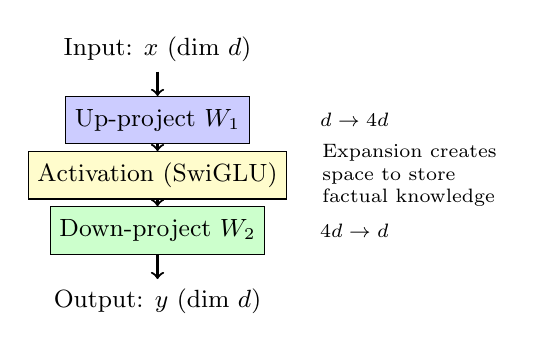
\begin{tikzpicture}[
    node distance=0.7cm,
    block/.style={rectangle, draw, minimum width=2cm, minimum height=0.6cm, font=\small},
    arrow/.style={->, thick}
]
% Input
\node (input) {\small Input: $x$ (dim $d$)};

% Expand
\node[block, fill=blue!20, below of=input, yshift=-0.2cm] (up) {Up-project $W_1$};
\node[right of=up, xshift=1.8cm, font=\scriptsize] {$d \rightarrow 4d$};

% Activation
\node[block, fill=yellow!20, below of=up] (act) {Activation (SwiGLU)};

% Contract
\node[block, fill=green!20, below of=act] (down) {Down-project $W_2$};
\node[right of=down, xshift=1.8cm, font=\scriptsize] {$4d \rightarrow d$};

% Output
\node[below of=down, yshift=-0.2cm] (output) {\small Output: $y$ (dim $d$)};

% Arrows
\draw[arrow] (input) -- (up);
\draw[arrow] (up) -- (act);
\draw[arrow] (act) -- (down);
\draw[arrow] (down) -- (output);

% Annotation
\node[right of=act, xshift=2.5cm, align=left, font=\scriptsize] {Expansion creates\\space to store\\factual knowledge};

\end{tikzpicture}
\caption{Feed-forward network: expand, activate, contract. Most parameters live here.}
\label{fig:ffn-structure}
\end{figure}
